\documentclass[tikz,border=8pt]{standalone}
\usepackage{amssymb}
\usepackage{pgfplots}
\pgfplotsset{compat=1.16}
\begin{document}
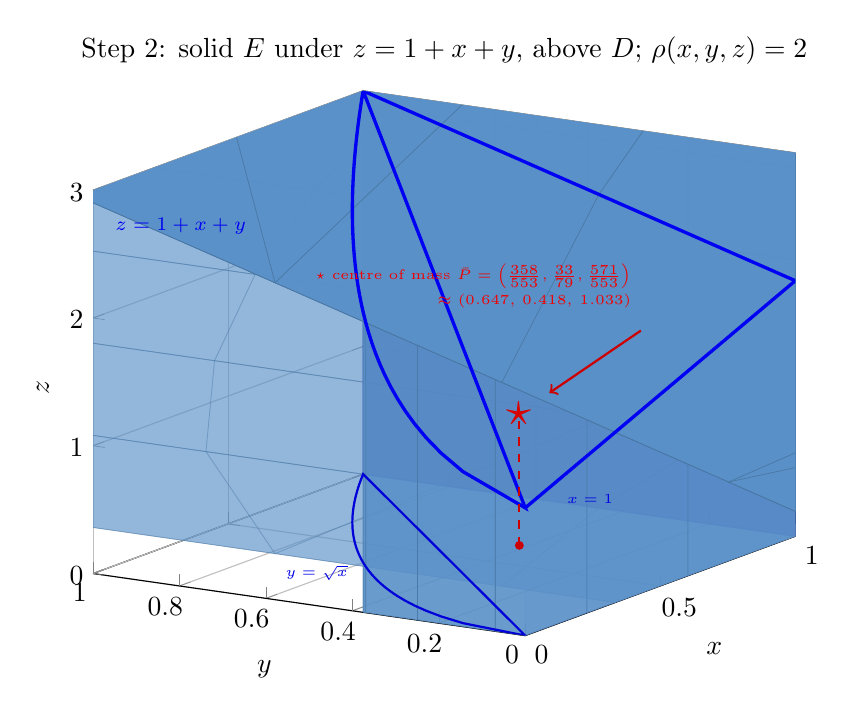
\begin{tikzpicture}
\begin{axis}[
    width=10.5cm, height=8.5cm,
    xlabel=$x$, ylabel=$y$, zlabel=$z$,
    xmin=0,xmax=1, ymin=0,ymax=1, zmin=0,zmax=3,
    view={-58}{17}, grid=major,
    title={Step 2: solid $E$ under $z=1+x+y$, above $D$; $\rho(x,y,z)=2$},
    colormap={cblue}{rgb255(0cm)=(90,145,200); rgb255(1cm)=(90,145,200)},
    point meta=1, point meta min=0, point meta max=1, shader=faceted,
]
% flat front wall over y = 0 (faint, so the interior stays visible)
\fill[blue!35!white, opacity=0.22, draw=blue!45, line width=0.25pt]
   (axis cs:0,0,0) -- (axis cs:1,0,0) -- (axis cs:1,0,2) -- (axis cs:0,0,1) -- cycle;
% base: region D in the plane z = 0
\addplot3[surf, opacity=0.30, samples=16, samples y=12, draw=blue!55, line width=0.25pt]
   ({x},{y*sqrt(x)},{0});
% flat side wall over x = 1
\fill[blue!60!black, opacity=0.55, draw=blue!85, line width=0.3pt]
   (axis cs:1,0,0) -- (axis cs:1,1,0) -- (axis cs:1,1,3) -- (axis cs:1,0,2) -- cycle;
% curved wall over y = sqrt(x)
\addplot3[surf, opacity=0.55, samples=16, samples y=8, draw=blue!80, line width=0.25pt]
   ({x},{sqrt(x)},{y*(1+x+sqrt(x))});
% top plane z = 1 + x + y over D
\addplot3[surf, opacity=0.85, samples=16, samples y=12, draw=blue!90, line width=0.25pt]
   ({x},{y*sqrt(x)},{1+x+y*sqrt(x)});
% key edges
\addplot3[very thick, blue!95!black, domain=0:1, samples=40] ({x},{sqrt(x)},{1+x+sqrt(x)});
\addplot3[very thick, blue!95!black, domain=0:1, samples=20] ({1},{x},{2+x});
\addplot3[very thick, blue!95!black, domain=0:1, samples=20] ({x},{0},{1+x});
\addplot3[thick, blue!85!black, domain=0:1, samples=40] ({x},{sqrt(x)},{0});
% centre of mass and its vertical fibre
\draw[red!80!black, thick, dashed] (axis cs:0.647,0.418,0) -- (axis cs:0.647,0.418,1.033);
\fill[red!80!black] (axis cs:0.647,0.418,0) circle (1.6pt);
\node[red!85!black, scale=1.8] (COM) at (axis cs:0.647,0.418,1.033) {$\star$};
\node[font=\tiny, blue!90!black] at (axis cs:1.04,0.50,0.02) {$x=1$};
\node[font=\tiny, blue!90!black] at (axis cs:0.22,0.62,0.02) {$y=\sqrt{x}$};
\node[font=\scriptsize, blue!95!black, anchor=west] at (axis cs:0.03,0.99,2.70) {$z=1+x+y$};
\node[font=\tiny, red!95!black, align=right, anchor=north east] at (axis cs:0.46,0.02,2.62)
      {$\star$ centre of mass $\bar P=\left(\frac{358}{553},\frac{33}{79},\frac{571}{553}\right)$\\[1pt]
       $\approx(0.647,\,0.418,\,1.033)$};
\draw[->, red!80!black, thick] (axis cs:0.46,0.02,2.02) -- (COM);
\end{axis}
\end{tikzpicture}
\end{document}
